\documentclass[ucs,blue,hyperref={pdfpagelabels=false},compress,handout]{beamer}

\mode<presentation>{
	%\usetheme{Berlin}
	%\usetheme{Frankfurt}
	%\usetheme{Warsaw}
	%\usetheme{Copenhagen}
	%\usetheme{Berkeley}
	%\usetheme{Luebeck}

%	\useoutertheme{infolines}

	%\usecolortheme{seahorse}

	%\setbeamercovered{transparent}

	\useoutertheme{split} % default / infolines
	\useoutertheme{nut} % default / infolines

	\useinnertheme{default}

	\usecolortheme{whale}
	%\usecolortheme{orchid}

	\setbeamerfont{block title}{size={}}

	%\setbeamertemplate{headline}[nut]
}

\usepackage[ngerman]{babel}
\usepackage[utf8x]{inputenc}
\usepackage{times}
\usepackage[T1]{fontenc}
\usepackage{multirow}
\usepackage{rotating}

\title[NUT: Netzwerkmanager für Linux]{NUT: Network UTility - ein Netzwerkmanager für Linux}
\date[\Today]{}

\author
[Daniel Bahrdt \and Stefan Bühler \and Oliver Groß]
{Daniel Bahrdt \and Stefan Bühler \and Oliver Groß \and \hbox{Betreuer: Dr. Boris Koldehofe}}

\hypersetup{pdfauthor={Daniel Bahrdt, Stefan Bühler, Oliver Groß}}

\pgfdeclareimage[height=2.5ex]{ul-logo}{institutmitlogo}
\pgfdeclareimage[height=2.5ex]{ur-logo}{qnut}
\pgfdeclareimage[height=1.5cm]{ilogo}{institutmitlogo}
\pgfdeclareimage[height=1.5cm]{plogo}{qnut}

\titlegraphic{\pgfuseimage{ilogo} \hskip 1cm \pgfuseimage{plogo}}

\institute
{
	Abteilung Verteilte Systeme \\
	Institut für Parallele und Verteilte Systeme \\
	Fakultät 5: Informatik, Elektrotechnik und Informationstechnik \\
	Universität Stuttgart
}

\homepage{http://repo.or.cz/w/nut.git}

\begin{document}

\begin{frame}
	\titlepage
\end{frame}

% \begin{frame}[<+-| alert@+>][t]{Überblick}
% 	\tableofcontents[pausesections,pausesubsections]
% \end{frame}

\section{Motivation}
\subsection{}
\begin{frame}[<+-| alert@+>]{Motivation}
	\begin{itemize}
		\item Konfiguration für ein Laptop in verschiedenen Arbeitsbereichen unpraktisch. \\
		\item Oft durch selbst zusammengehackte Skripte erleichtert, die meist aber mit ``sudo'' ausgeführt werden müssen.
		\item Umständliches Starten aller notwendigen Teile (WLAN Konfigurieren, IP zuweisen, VPN aufbauen)
		\item Unflexibel: Je nach Umgebung andere Konfiguration nötig
	\end{itemize}
\end{frame}

\begin{frame}[fragile]{Motivation-Beispielskript}
\fontsize{4.8}{5.8} \selectfont
\begin{verbatim}
#!/bin/bash
echo "* loading modules...";
echo "  -> acer_acpi";
modprobe -r acer_acpi;
modprobe acer_acpi;
if [ "$1" = "bcm" ]
then
    echo "  -> bcm43xx";
    modprobe bcm43xx;
else
    echo "  -> ndiswrapper";
    modprobe ndiswrapper;
fi
echo "* enabling wlan hardware...";
echo "enabled: 1" > /proc/acpi/acer/wireless;
sleep 0.1;
if [ "$1" = "bcm" ]
then
    iwconfig wlan0 rate 11M;
fi
echo "* bringing up wlan interface...";
if [ "$2" = "connect" -o "$1" = "connect" ]
then
    ifup wlan0;
elif [ "$2" = "connect2" -o "$1" = "connect2" ]
then
    echo "* starting wpa supplicant...";
    wpa_supplicant -B -i wlan0 -D wext -c /etc/wpa_supplicant/wpa_supplicant.conf;
    sleep 1;
    echo "* starting dhcp client"
    dhclient wlan0
fi
\end{verbatim}
\end{frame}

\begin{frame}[<+-| alert@+>]{Überblick NUt}
	\begin{itemize}
		\item nuts: Daemon(Server) zur Verwaltung der Hardware
		\item libnutclient: Abstraktion der Kommunikation mit dem Server
		\item libnutwireless: Abstraktion der Kommunikation mit dem wpa\_supplicant
		\item QNut: Grafische Benutzeroberfläche in Qt
		\item Genutzte Frameworks/Libraries: Qt4, dbus, libnl, iwlib
	\end{itemize}
\end{frame}


\section{Server}
\subsection{Aufbau}
\begin{frame}[<+-|alert@+>]{Überblick der Strukturen}
	\includegraphics<+->{nutsstructure.pdf}
	\begin{itemize}
		\item Devices: Entsprechen den Hardwaregeräten
		\begin{itemize}
			\item Erkennt Zustandsänderungen wie Kabel ein-/ausstecken oder WLAN Verbindung.
			\item Kann für WLAN Karten den wpa\_supplicant automatisch starten und beenden.
		\end{itemize}
		\item Environments: Entsprechen Umgebungen; z.Bsp. Arbeitsplatz, Zuhause, ...
		\item Interfaces: Entsprechen je einer IP
	\end{itemize}
\end{frame}

\begin{frame}[<+-|alert@+>]{Environment}
	\begin{itemize}
		\item Environments werden je nach Konfiguration vom Server automatisch ausgewählt, Kriterien für die Auswahl sind:
		\begin{itemize}
			\item Der WLAN Name, in dem sich das Device befindet (ESSID)
			\item Das Vorhandenseins eines Rechners mit einer bestimmten IP (und evtl. passender MAC Adresse)
			\item Wunsch des Benutzers.
		\end{itemize}
	\end{itemize}
\end{frame}

\begin{frame}[<+-|alert@+>]{IP Zuweisung}
	\begin{itemize}
		\item 3 verschiedene Methoden:
		\begin{itemize}
			\item Statisch konfigurierte (oder vom Benutzer eingegebene) IP
			\item Per DHCP (benötigt einen DHCP-Server)
			\item Zeroconf (aka \href{http://tools.ietf.org/html/rfc3927}{``IPv4 Link-Local Adresses'', RFC 3927});
				es wird eine lokal freie IP aus dem Bereich 169.254/16 gesucht. Die IP ist nur im lokalen Netzwerk gültig.
		\end{itemize}
		\item Zur IP gehören weitere Werte, die auch pro Interface konfiguriert werden: Netmask, Gateway, DNS-Server.
	\end{itemize}
\end{frame}

\subsection{Weitere Features}
\begin{frame}[<+-|alert@+>]{Weitere Features}
	\begin{itemize}
		\item Eventgesteurte Scriptausführung: das ermöglich z.Bsp. den Aufbau eines VPN nach dem Aufbau der darunterliegenden Verbindung (die Skripte haben Rootrechte)
		\item Unterstützt Plug'n'Play von Netzwerkgeräten, z.Bsp. PCMCIA Karten oder Laden und Entladen von Treibern wegen Inkompatibilität mit Suspend.
	\end{itemize}
\end{frame}

\subsection{Beispiel}
\begin{frame}[fragile]{Konfigurationsbeispiel 1}
\tiny
\begin{verbatim}
device "eth0" {
    no-auto-start; //Nicht beim starten von nuts aktivieren
    dhcp; //Default environment dhcp (optional)
    environment "zeroconf" zeroconf; //Zeroconf environment
    environment "userdefineable" static user; //Environment mit benutzerdefinierbarem Interface
    // Environment wird nach einer IP-Adresse in Verbindung mit MAC (optional) ausgewählt
    environment "home" select arp 192.168.0.1 00:07:40:EC:D0:BE;
};
device "eth1" {
    wpa-supplicant config "/etc/wpa_supplicant/wpa_supplicant.conf" driver "wext";
    dhcp;
    environment "infeap" {
        select essid "infeap";
    };
    environment "static/dynamic" {
        dhcp;
        static {
            ip 192.168.0.61;
            netmask 255.255.255.0;
            gateway 192.168.0.1;
            dns-server 192.168.0.1;
        };
    };
    environment "zeroconf" {
        zeroconf;
    };
};
\end{verbatim}
\end{frame}

\begin{frame}[fragile]{Konfigurationsbeispiel 2}
\fontsize{4.8}{5.8} \selectfont
\begin{verbatim}
device "eth1" {
    wpa-supplicant config "/etc/wpa_supplicant/wpa_supplicant.conf" driver "wext";
    dhcp;
    environment "infeap" {
        select essid "infeap";
    };
    environment "home" {
        dhcp;
        select or {
            select and {
                essid "buftop";
                arp 192.168.0.1 00:07:40:EC:D0:BE;
            };
            select and {
                essid "unten";
                arp 192.168.178.1 00:15:0C:46:2D:C7;
            };
        };
    };
    environment "static/dynamic" {
        dhcp;
        static {
            ip 192.168.0.61;
            netmask 255.255.255.0;
            gateway 192.168.0.1;
            dns-server 192.168.0.1;
        };
    };
    environment "zeroconf" {
        zeroconf;
    };
};
\end{verbatim}
\end{frame}


% TODO
\section{Library}
\subsection{libnutclient}
\begin{frame}[<+-| alert@+>]{nut client}
	\begin{itemize}
		\item Qt-Library für den Client-Teil der DBus Verbindung zum Server.
	\end{itemize}
\end{frame}

\subsection{libnutwireless}
\begin{frame}[<+-| alert@+>]{wireless client}
	\begin{itemize}
		\item Qt-Library für die wpa\_supplicant Verwaltung.
	\end{itemize}
\end{frame}


% TODO
\section{Client}
\subsection{Überblick}
\begin{frame}[<+-| alert@+>]{QNut}
	\begin{itemize}
		\item nahezu vollständige Steuerung des Servers über die Library
		\item Steuerung des wpa\_supplicant ebenfalls über die Library
		\item benutzerspezifische Skripte möglich
		\item Feedback für den Benutzer
	\end{itemize}
\end{frame}


\subsection{QNut}
\begin{frame}[<+-| alert@+>]{Hauptfenster}

		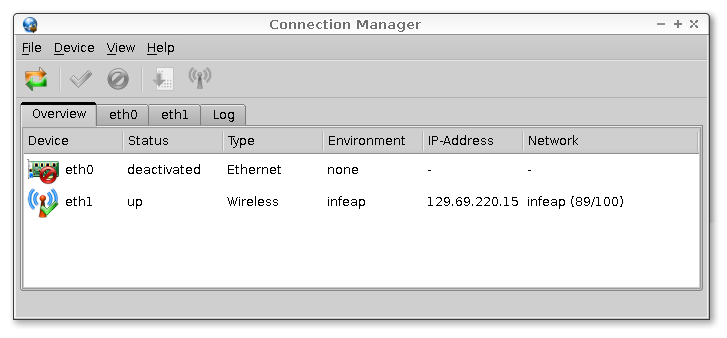
\includegraphics[scale=0.25]{qnut_overview.png}
		% qnut_overview.png: 727x338 pixel, 72dpi, 25.65x11.92 cm, bb=0 0 727 338

	\begin{itemize}
		\item Übersichten für Devices, Environments und Drahtlosnetzen
		\item Aktueller Status
	\end{itemize}
\end{frame}

\begin{frame}[<+-| alert@+>]{Steuerung und Skripte}

		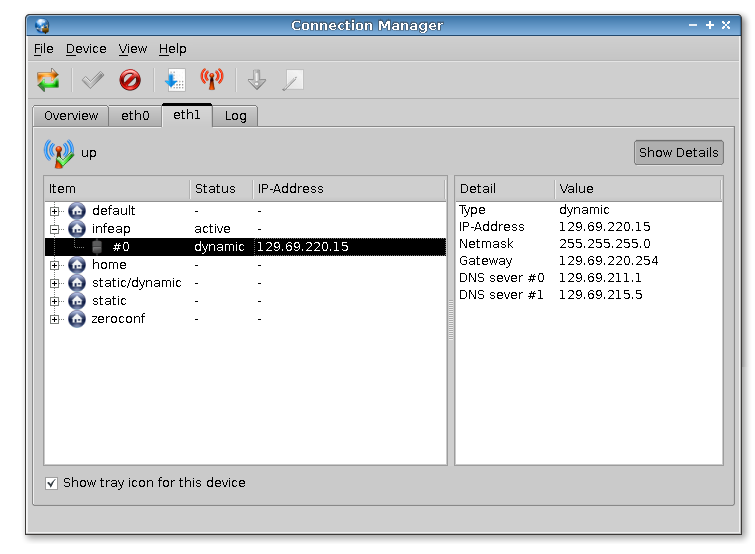
\includegraphics[scale=0.25]{qnut_detailed.png}
		% qnut_detailed.png: 755x554 pixel, 72dpi, 26.63x19.54 cm, bb=0 0 755 554

	\begin{itemize}
		\item Detailansichten für Environments und Interfaces
		\item Auswahl eines aktiven Environments
		\item Konfiguration eines Interaces
	\end{itemize}
\end{frame}

\begin{frame}[<+-| alert@+>]{Steuerung und Skripte}

		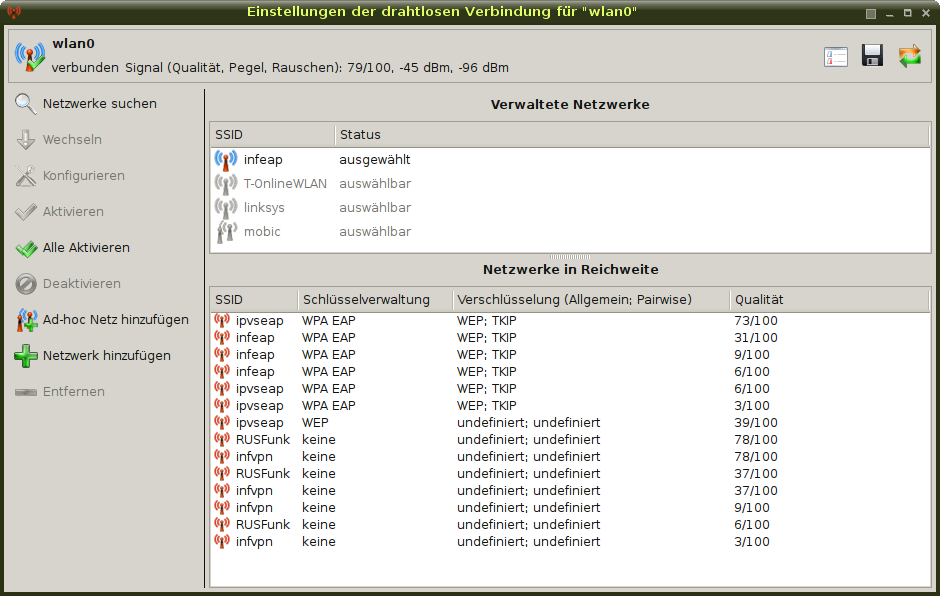
\includegraphics[scale=0.25]{qnut_scan.png}
		% qnut_scan.png: 952x651 pixel, 72dpi, 33.58x22.97 cm, bb=0 0 952 651

	\begin{itemize}
		\item Anpassung der verwalteten Drahtlosnetze
		\item Scannen nach vorhandenen Drahtlosnetzen
	\end{itemize}
\end{frame}

\begin{frame}[<+-| alert@+>]{Steuerung und Skripte}

		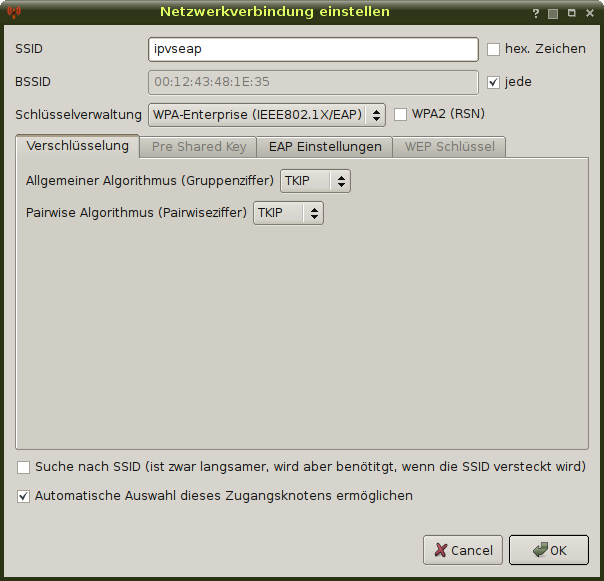
\includegraphics[scale=0.25]{qnut_netconfig.png}
		% qnut_netconfig.png: 523x602 pixel, 72dpi, 18.45x21.24 cm, bb=0 0 523 602

	\begin{itemize}
		\item Hinzufügen und Entfernen von Drahtlosnetzen
		\item Konfiguration vorhandener Netzwerke
	\end{itemize}
\end{frame}


\begin{frame}[<+-| alert@+>]{Sonstiges}

	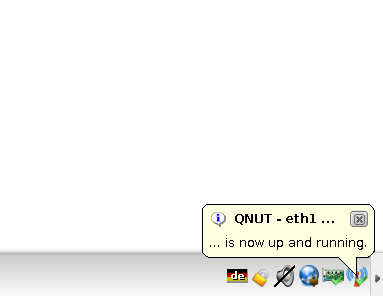
\includegraphics[scale=0.25]{qnut_tooltip.png}
	% qnut_tooltip.png: 383x296 pixel, 72dpi, 13.51x10.44 cm, bb=0 0 383 296

	\begin{itemize}
		\item Tray-Icon zum schnelleren Zugang
		\item Statusänderung der Devices als Tool-Tip
		\item Ausführung von Skripten je Devicestatus
	\end{itemize}
\end{frame}





\section{Zusammenfassung}
\subsection{Konkurrenz}
\begin{frame}{Andere Netzwerkmanager}
	\fontsize{7}{8.4}\selectfont
	\begin{center}
	\begin{tabular}{cc|c|c|c|c|c}
		&					& kwifi		& gtkwifi	& wifi radar	& NetworkManager	& NUt \\
		\hline
		&Environments		& $X$			& $X$			& $X$			& $X$				& $\surd$ \\
		\hline
		\multirow{3}{*}{\begin{sideways} Gerät \end{sideways}}
		& Ethernet			& $X$			& $X$			& $X$			& $\surd$			& $\surd$ \\
		\cline{2-7}
		& Drahtlos			& $\surd$		& $\surd$		& $\surd$		& $\surd$			& $\surd$ \\
		\cline{2-7}
		& PPP				& $X$			& $X$			& $X$			& $\surd$			& $X^{4}$ \\
		\hline
		\multirow{3}{*}{\begin{sideways} IP-Konf. \end{sideways}}
		&static				& $\surd$		& $\surd$		& $\surd$		& $\surd$			& $\surd$ \\
		\cline{2-7}
		& dhcp				& $\surd$		& $\surd$		& $\surd$		& $\surd$			& $\surd$ \\
		\cline{2-7}
		& zeroconf			& $X$			& $X$			& $X$			& $\surd$			& $\surd$ \\
		\hline
		\multirow{4}{*}{\begin{sideways} WLAN \end{sideways}}
		&unverschlüsselt	& $\surd$		& $\surd$		& $\surd$		& $\surd$			& $\surd^{3}$ \\
		\cline{2-7}
		&WEP				& $\surd$		& $\surd$		& $\surd$		& $\surd$			& $\surd^{3}$ \\
		\cline{2-7}
		&WPA				& $\surd$		& $\surd$		& $\surd$		& $\surd$			& $\surd^{3}$ \\
		\cline{2-7}
		&Konfig. speichern	& $\surd^{5}$	& $\surd^{5}$	& $\surd^{5}$	& $\surd^{5}$		& $\surd^{3}$
	\end{tabular}
	\end{center}
	\begin{itemize}
		\item[1] built-in
		\item[2] external
		\item[3] über wpa\_supplicant
		\item[4] mit Skripten möglich aber nicht als Konfigurationsoption verfügbar
		\item[5] eigene
	\end{itemize}
\end{frame}

\begin{frame}[<+-| alert@+>]{Motivation-NetworkManager<=>NUt}
	\begin{tabular}{l|c|c}
								& NetworkManager	& NUt \\
		\hline
		Environments			& $X$					& $\surd$ \\
		\hline
		Server-Skripte			& $X$					& $\surd$ \\
		\hline
		Nutzer-Skripte			& $X$					& $\surd$ \\
		\hline
		QT-GUI					& $\surd$(KDE3)			& $\surd$(Qt4) \\
		\hline
		GTK-GUI					& $\surd$(Gnome)		& $X$			\\
		\hline
		DBus-Interface			& $\surd$				& $\surd$	\\
		\hline
		Client-Library			& $X$					& $\surd$(Qt4)	\\
		\hline
		Autom. Netzwechsel		& $\surd$				& nur pro Gerät \\
		\hline
		Plugin-Struktur			& $\surd$				& $X$
	\end{tabular}
\end{frame}


\subsection{Zukünftiges}
\begin{frame}[<+-|alert@+>]{Mögliche zukünftige Änderungen}
	\begin{itemize}
		\item Bugfixes (sofern weitere nötig)
		\item Server
		\begin{itemize}
			\item Fallback-Konfiguration für DHCP
			\item Signal vom Server falls ein neues Netzwek gefunden wurde
			\item PPP als Konfigurationsoption (momentan nur über Skripte)
		\end{itemize}
		\item libnut/qnut
		\begin{itemize}
			\item Etwas mehr Unabhängigkeit vom wpa\_supplicant
			\item Mehr WLAN-Informationen (z.B. Übertragungsgeschwindigkeit)
		\end{itemize}
		\item Sehr zukünftiges
		\begin{itemize}
			\item DBus Interface generischer machen
			\item Konsolenclient
			\item IPv6
		\end{itemize}
	\end{itemize}
\end{frame}

\subsection{Fazit}
\begin{frame}[<+-|alert@+>]{Warum brauche ich NUt?}
	\begin{itemize}
		\item Es ist kostenlos (GPL)
		\item Es ist schnell
		\item Es verbraucht wenig Speicher und keine CPU-Zeit (im Idle)
		\item Es steuert alle gängigen vom wpa\_supplicant unterstützten
		\item Es steuert alle Netzwerkadapter an
		\item Es ist durch die Skripte enorm flexibel
	\end{itemize}
\end{frame}

\begin{frame}[<+-|alert@+>]{Ende}
	\begin{center}
		\begin{Large}
			Homepage, Debuild Skripte und Ebuild:
		\end{Large}
		\begin{Huge}
			http://repo.or.cz/w/nut.git
		\end{Huge}
	\end{center}
\end{frame}


\end{document}
